% !TEX TS-program = xelatex
% !TEX encoding = UTF-8 Unicode

% Tennessee Technological University
% ME4140 - Fall 2016 - Fall 2017 - ? - Fall 2019 - Fall 2020
% Tristan Hill - September 19, 2020 - October 09, 2020
% Turtorial 6 - Turtlebot3 Navigationw

\documentclass[12pt]{article}

% Custom Preamble
\usepackage{/home/thill/Documents/lectures/ros_workshop/ros_tutorial} 

% Title and Misc
\newcommand{\MNUM}{6} %Module Number
\newcommand{\MNAME}{Turtlebot3 Simulator} %Module Name
\pagestyle{myheadings}
\markright{{\large ME4140 - ROS Workshop - Fall 2020}}

%\newcommand{\pkgname}{<package\_name>}
%\newcommand{\wspname}{<workspace\_name>}
%\newcommand{\nodname}{<node\_name>}
%\newcommand{\tpcname}{<topic\_name>}
%\newcommand{\lfname}{<file\_name>}
%\newcommand{\home}{\textasciitilde/}
%\newcommand{\rosdistro}{melodic}
%\newcommand{\pthname}{/opt/ros/\rosdistro/share/turtlebot\_stage/maps/}


\begin{document}

\thispagestyle{plain}

\begin{center}
   {\bf \Large ROS - Navigation and The Turtlebot3 Simulator}\vspace{2mm} \\
   {\bf \large ME 4140 - Introduction to Robotics - Fall 2020} \\
\end{center}


What do we mean by navigation? This means different things in different places. Here, we mean the navigation stack in ROS melodic. This tutorial comes from \href{http://emanual.robotis.com/docs/en/platform/turtlebot3/simulation/#simulation} {here.}  \\

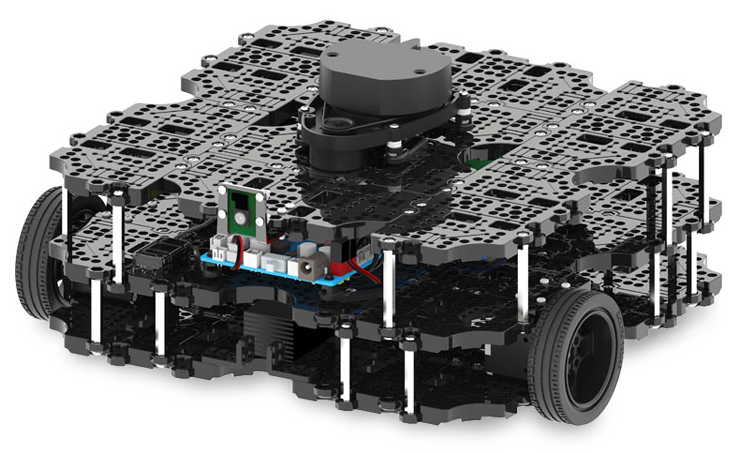
\includegraphics[scale=.25]{turtlebotPi.jpg}
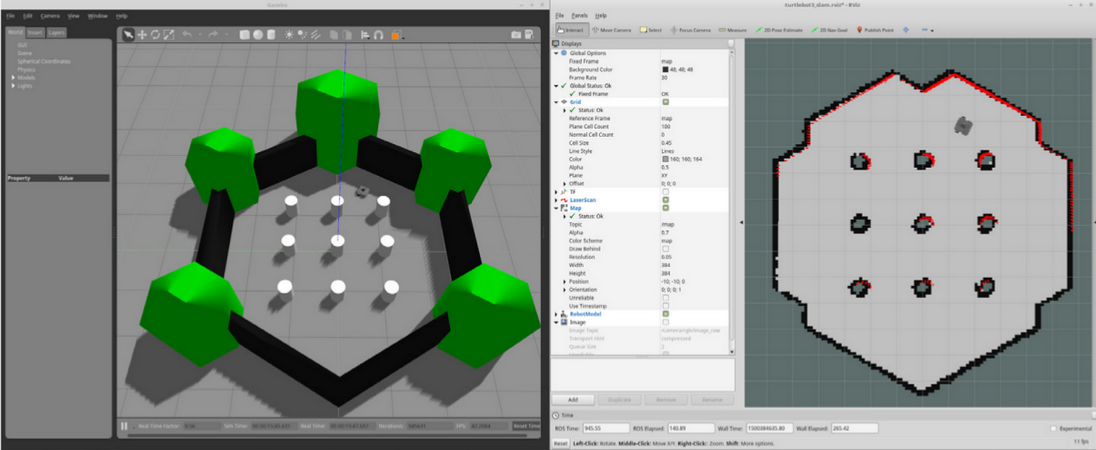
\includegraphics[scale=.3]{turtlebot3_maps.png} 

\begin{description}[labelindent=1cm]
	
	\item[\textbf{\underline{Overview:}}] \hfill \vspace{3mm}\\
	After completing {\it Tutorial 5 - Turtlebot Simulator}, You have learned some basics of ROS, and you have a for a more advanced robot. Next you are going to learn to use the navigation stack with the turtlebot3 simulator. Read more \href{https://emanual.robotis.com/docs/en/platform/turtlebot3/navigation/#ros-1-navigation}{here} and \href{http://wiki.ros.org/navigation/Tutorials}{here}.
	
	\item[\textbf{\underline{System Requirements:}}] \hfill \vspace{0mm}

\begin{itemize}
	\item {\bf ROS+OS}: This tutorial is intended for a system with ROS Melodic installed on the Ubuntu 18.04 LTS operating system. Alternate versions of ROS (i.e. - Kinetic, Noetic, etc.) may work but have not been tested. Versions of ROS are tied to versions of Ubuntu.
	\item {\bf ROS:} Your computer must be connected to the internet to proceed. Update the system before you begin.
	\item {\bf Workspace Setup:} The Turtlebot3 Simulator from tutorial 5 must be operational before completing tutorial 6.  
\end{itemize}

	
	\item[\textbf{\underline{Disclaimer:}}] \hfill \vspace{0mm}
	
	\begin{itemize}

		\item {\R\underline{\bf Backup the System:}} If you are using a virtual machine, it is recommend to make a snaphot of your virtual machine before you start each module. In the event of an untraceable error, you can restore to a previous snapshot. 
		
		\item \underline{\B ROSLAUNCH:} This tutorial involves using the roslaunch command which runs a muliple of nodes at once as described in the launch file. We will learn more about this later. 
	
		\item \underline{\G Mouse for 3D viewing:} This simulator view is much easier use if you have a three button mouse plugged in, but this is not required.
	
		 
	\end{itemize}


\newpage
\item[\textbf{\underline{Part 1 - Install navigation and gmapping packges:}}] \hfill \vspace{0mm}
	
\begin{enumerate}
\item {\bf Install the {\bf navigation} and {\bf gmapping} nodes if you have not already.}
\begin{minted}{text} 
sudo apt install ros-melodic-navigation ros-melodic-gmapping
\end{minted}

\item {\bf Set the robot model. This only needs to be done once. Modify the .bashrc file If you want to change models. }
\begin{minted}{text}
echo "export TURTLEBOT3_MODEL=waffle_pi" >> ~/.bashrc
source ~/.bashrc
\end{minted}

\end{enumerate}

\item[\textbf{\underline{Part 2 - Generate a map of the virtual space:}}] \hfill \vspace{0mm}	\\

\begin{enumerate}
\item {\bf   Start the turtlebot3 simulator.}
\begin{minted}{text} 
roslaunch turtlebot3_gazebo turtlebot3_world.launch
\end{minted}
\item {\bf Next, start SLAM using the gmapping node. }
\begin{minted}{text} 
roslaunch turtlebot3_slam turtlebot3_slam.launch slam_methods:=gmapping
\end{minted}
\item {\bf Drive the robot around with the keyboard to collect pose and Lidar data}
\begin{minted}{text} 
roslaunch turtlebot3_teleop turtlebot3_teleop_key.launch
\end{minted}
\item {\bf When you are finished save the map. (-f allows the filename to be set)}
\begin{minted}{text} 
rosrun map_server map_saver -f map
\end{minted}

Two map files (.pgm and .yaml) will appear in the current folder after Step 4. If you move the map to a new directory, keep both files together.

\end{enumerate}


%    \item Next install the physical 'turtlebot' drivers into your ROS system. This step is only necessary if you are using a real turtlebot. \href{http://wiki.ros.org/Robots/TurtleBot} {Link Here} 
%   \begin{minted}{text}  
%(sudo apt-get install ros-|\rosdistro|-turtlebot ros-|\rosdistro|-turtlebot-apps
%ros-|\rosdistro|-turtlebot-interactions ros-|\rosdistro|-turtlebot-simulator 
%ros-|\rosdistro|-kobuki-ftdi ros-|\rosdistro|-rocon-remocon 
%ros-|\rosdistro|-rocon-qt-library ros-|\rosdistro|-ar-track-alvar-msgs})
%\end{minted}
%    
\newpage
\item[\textbf{\underline{Part 3 - Navigate the virtual space using the map and RVIZ:}}] \hfill \vspace{2mm}	\\
Now that navigation is installed and there is a map saved to file, the robot can perform\\ autonomous point to point navigation with dynamic obstacle avoidance. \\
\begin{enumerate}
\item {\bf   Start the turtlebot3 simulator.}
\begin{minted}{text} 
  roslaunch turtlebot3_gazebo turtlebot3_world.launch
\end{minted}
\item {\bf  Turn on the navigation nodes and RVIZ. Use the name of the map you created. }
\begin{minted}{text} 
roslaunch turtlebot3_navigation turtlebot3_navigation.launch map_file:=map.yaml
\end{minted}

	The gazebo window will open containing your robot, and you will also see the rviz window open separately. Find and test the following features of navigation in RVIZ. \\
	
	1) \underline{Pose Estimate} - Click and drag the direction to set the current pose estimate of the robot. \vspace{2mm} \\
	
	2) \underline{2D Nav Goal} - Click and drag the direction to define a goal point for the robot in the map. \vspace{2mm} \\

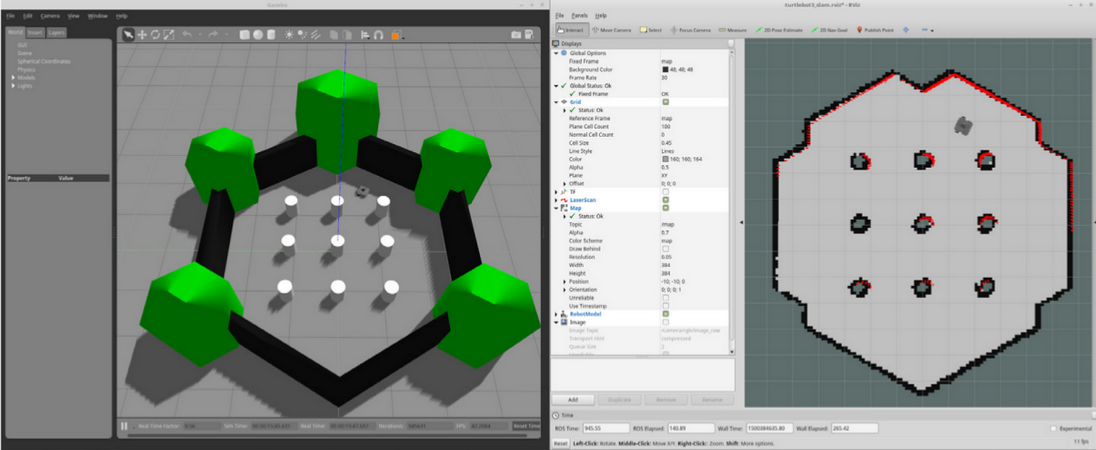
\includegraphics[scale=.350]{turtlebot3_rviz.png}



\item {\bf Check the available topics with rostopic. }
\begin{minted}{text} 
rostopic list
\end{minted}
\begin{minted}{text} 
rosrun rqt_graph rqt_graph 
\end{minted}

\end{enumerate}

\newpage
\item[\textbf{\underline{Part 4 - Issues Loading Maps Files:}}] \hfill \vspace{2mm}	\\

You may have run into an issue in which {\it turtlebot3\_navigation} cannot load the map file. A typical error message is shown below, along with with the preferred solution.


\color{red}
\begin{minted}{text} 

[ERROR] [1604667817.760623311]: Map server could not open /map.yaml.

\end{minted}
\color{black}

\begin{itemize}

\item Leave the top line of {\it map.yaml } as is when the file is generated. Do not add the full path to map file. The filename is sufficient. 

\item Copy {\it map.yaml } and {\it map.pgm } to the maps/ directory of a package in the ROS workspace.

\item Ensure that the workspace will compile and build with {\it catkin\_make}. You should see in the terminal output, that your package was successfully built. 

\item Finally, use the {\it find} command to point the node to the maps directory of your package.

\end{itemize}

Now repeat the commands from before with the addition of the find command in the map argument. 

\begin{enumerate}


\item {\bf   Start the turtlebot3 simulator.}
\begin{minted}{text} 
  roslaunch turtlebot3_gazebo turtlebot3_world.launch
\end{minted}
\item {\bf  Turn on the navigation nodes and RVIZ. Use the name of the map you created. }

\begin{framed}
\begin{verbatim}

roslaunch turtlebot3_navigation turtlebot3_navigation.launch \
map_file:='$(find <YOUR PKG>)\maps\<YOUR MAP>.yaml'

\end{verbatim}
\end{framed}




\end{enumerate}

\vspace{100mm}

\item[\textbf{\underline{Tutorial Complete:}}] \hfill \vspace{3mm}\\ 
	After completing {\it Tutorial 6 - Turtlebot3 Simulator}, you are ready to learn about ... more ROS!
	
	\hspace {30mm}	
	
	
	
	
\includegraphics[scale=.350]{../../charlie_robot.jpeg} \vspace{5mm}\\
    \LARGE \textbf{NOW, YOU KNOW ABOUT ROS! GOOD JOB!}
	
	
		 

%    \begin{itemize}
%    
%        \item {\fontfamily{qcr}\selectfont  \hspace{5mm} \pthname maze.png}
%        \item {\fontfamily{qcr}\selectfont  \hspace{5mm} \pthname maze.yaml}
%        \item {\fontfamily{qcr}\selectfont  \hspace{5mm} \pthname stage/maze.world}
%    
%    \end{itemize}

%    \item First try the simulator in the demo world called {\it maze}. We will export the files as {\it environment variables}
%
%    {\fontfamily{qcr}\selectfont  \hspace{5mm} \$ export TURTLEBOT\_STAGE\_MAP\_FILE=\\"\pthname maze.yaml"}\\
% 
%    {\fontfamily{qcr}\selectfont  \hspace{5mm} \$ export TURTLEBOT\_STAGE\_WORLD\_FILE=\\"\pthname stage/maze.world"}\\
%    
%    \item Now use the launch file (available upon install) to start the simulator.\\
%    {\fontfamily{qcr}\selectfont  \hspace{5mm} \$ roslaunch turtlebot\_stage turtlebot\_in\_stage.launch}
%    
%    \item Now you can modify the world you have just simulated. To do this copy all three files and rename them something sensible. Open the {\it .png} file with any image editor, and draw on it and save. You also need to modify just a few lines in the {\it .yaml} file and the {\it .world} file. (Note: This step will be detailed in the next tutorial. Continue at your own risk or contact me for help.)
%    
%     \item Did you notice an error when you turned the node on? We can fix that.  \\\\
%    
%    	 {\fontfamily{qcr}\selectfont  \hspace{5mm} \$ sudo  gedit /opt/ros/\rosdistro/share/gmapping/nodelet\_plugins.xml}\\\\
%    	 
%    	 Copy the code below into the new file. This a bug related to moving to `kinetic'.\\
%    \lstset{language=XML}
%     \begin{lstlisting}
%
%<library path="lib/libslam_gmapping_nodelet">
%    <class name="SlamGMappingNodelet" type="SlamGMappingNodelet" base_class_type="nodelet::Nodelet">
%        <description>
%            Nodelet ROS wrapper for OpenSlams Gmapping.
%        </description>
%    </class>
%</library>
%      \end{lstlisting}
%
%\vspace{5mm}    Now run your node again.

\end{description}
\end{document}

